% Opening packages ---------------------------------

\documentclass[12pt, a4paper]{article}
\parindent 0px
\parskip=10pt
\usepackage[utf8]{vietnam}
\usepackage[left=1.20cm, right=1.20cm, top=1.50cm, bottom=1.50cm]{geometry}
\usepackage{amsmath,amssymb,amsfonts}
\usepackage{gensymb}
\usepackage{enumitem}
\usepackage{multicol}
\usepackage{graphicx}
\usepackage{array}
\usepackage{float}
\usepackage[onehalfspacing]{setspace}
\usepackage{mathpazo}
\usepackage{wrapfig}
\usepackage{tkz-tab}

% Title --------------------------------------------


\title{\vspace{-1.5cm}{\huge\textbf{Ôn thi cuối kỳ I - Lần 1}}\\[3mm]
		{\LARGE Khối lớp: 12}\\[2mm]
{\normalsize Họ và tên~\rule{3cm}{1pt} \hfill Ngày nhận đề: ~\rule{3cm}{1pt}}\\[4mm]
\hrule
}
\author{}
\date{}

% Bắt đầu đề---------------------------------------

\begin{document}
	\maketitle
	\vspace{-2.15cm}
	
\textbf{Phần I. Câu hỏi trắc nghiệm nhiều phương án lựa chọn}

\textbf{Câu 1: } Cho hình hộp $ ABCD.A'B'C'D' $. Đẳng thức nào sau đây \textbf{sai}?
	\begin{multicols}{2}
		\begin{enumerate}
			\item[\textbf{A.}] $ \overrightarrow{AB} + \overrightarrow{AD} = \overrightarrow{AC} $
			\item[\textbf{C.}] $ \overrightarrow{AC} + \overrightarrow{BB'} = \overrightarrow{AC'} $
			\item[\textbf{B.}] $ \overrightarrow{AD} + \overrightarrow{CC'} = \overrightarrow{AD'} $
			\item[\textbf{D.}] $ \overrightarrow{AB'} + \overrightarrow{CB} = \overrightarrow{AC'} $
		\end{enumerate}
	\end{multicols}
	
\vspace{-1cm}

\begin{minipage}{0.7\textwidth}
    \noindent
    \textbf{Câu 2:} Cho hàm số $y = \dfrac{ax^2 + bx + c}{mx + n}$ \, $(\text{với } a \neq 0; \, m \neq 0)$ có đồ thị như hình vẽ bên dưới đây. Phương trình đường tiệm cận xiên của đồ thị hàm số đã cho là:
    
    % Hai cột đáp án
    \begin{multicols}{2}
        \begin{enumerate}
            \item[\textbf{A.}] $y = x - 2$
            \item[\textbf{B.}] $y = 2x + 2$
            \item[\textbf{C.}] $y = 2x - 2$
            \item[\textbf{D.}] $y = x + 2$
        \end{enumerate}
    \end{multicols}
\end{minipage}%
\hfill
\begin{minipage}{0.3\textwidth}
    \centering
    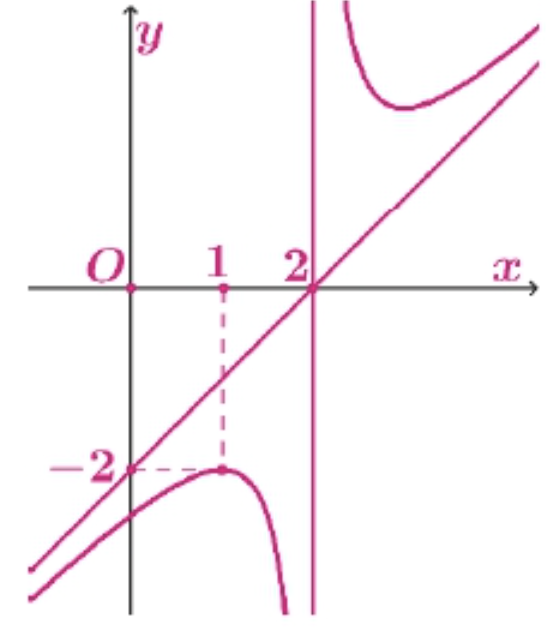
\includegraphics[scale=0.45]{../assets/1.png} % Thay "1" bằng tên file hình ảnh
\end{minipage}

\textbf{Câu 3: } Theo thống kê điểm trung bình môn Toán của một số học sinh đã trúng tuyển vài lớp 10 năm học 2024 - 2025 của Trường THPT Lê Quý Đôn được kết quả như bảng sau:
\vspace{-0.4cm}
	\begin{center}
		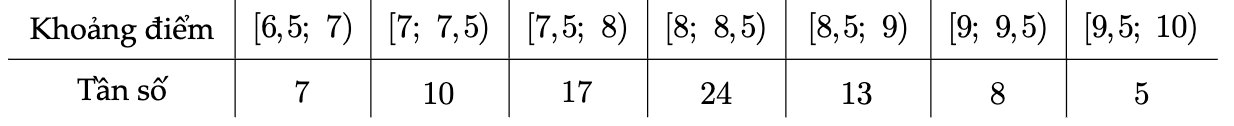
\includegraphics[scale=0.75]{../assets/2.png}
	\end{center}
\vspace{-0.8cm}
	Khoảng tứ phân vị của mẫu số liệu ghép nhóm trên là
	\begin{multicols}{4}
		\begin{enumerate}
			\item[\textbf{A.}] $ \Delta _Q = 1,1 $
			\item[\textbf{B.}] $ \Delta _Q = 1 $
			\item[\textbf{C.}] $ \Delta _Q = 1,2 $
			\item[\textbf{D.}] $ \Delta _Q = 0,6 $
		\end{enumerate}
	\end{multicols}
	
\textbf{Câu 4: } Cho hàm số bậc ba có bảng biến thiên như hình vẽ dưới đây. Giá trị cực tiểu của hàm số là:
	\begin{center}
			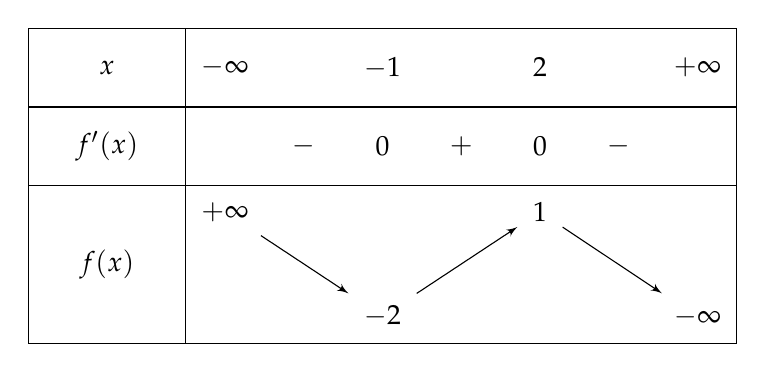
\begin{tikzpicture}
				\tkzTabInit[nocadre = false , lgt = 2 , espcl = 2]
					{ $ x $ / 1 , $ f'(x) $ / 1 , $ f(x) $ / 2 }
					{ $ - \infty $ , $ -1 $ , $ 2 $ , $ + \infty $ } 
				\tkzTabLine
					{ , - , $ 0 $ , + , $ 0 $ , - , }
				\tkzTabVar
					{ +/ $ +\infty $ , -/ $ -2 $ , +/ $ 1 $ , -/ $ -\infty $ }
			\end{tikzpicture}
	\end{center}
	\begin{multicols}{4}
		\begin{enumerate}
			\item[\textbf{A.}] $ 1 $
			\item[\textbf{B.}] $ -2 $
			\item[\textbf{C.}] $ 2 $
			\item[\textbf{D.}] $ -1 $
		\end{enumerate}
	\end{multicols}
	
\pagebreak

\textbf{Câu 5: } Cho tứ diện $ ABCD $ có $ G $ là trọng tâm tam giác $ BCD $. Véc tơ $ \overrightarrow{AB} + \overrightarrow{AC} + \overrightarrow{AD} $ bằng
	\begin{multicols}{4}
		\begin{enumerate}
			\item[\textbf{A.}] $ 3\overrightarrow{AG} $
			\item[\textbf{B.}] $ \overrightarrow{AG} $
			\item[\textbf{C.}] $ 3\overrightarrow{DG} $
			\item[\textbf{D.}] $ 2\overrightarrow{AG} $
		\end{enumerate}
	\end{multicols}
	
\textbf{Câu 6: } Thống kê điểm thi tốt nghiệp môn toán THPT năm 2025 của lớp 12A tại một trường THPT thu được kết quả như sau:
\vspace{-0.4cm}
	\begin{center}
		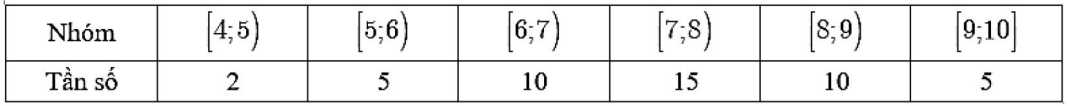
\includegraphics[scale=0.85]{../assets/3.png}
	\end{center}
\vspace{-0.7cm}
	Khoảng biến thiên của mẫu số liệu thống kê trên là
	\begin{multicols}{4}
		\begin{enumerate}
			\item[\textbf{A.}] $ 13 $
			\item[\textbf{B.}] $ 6 $
			\item[\textbf{C.}] $ 7 $
			\item[\textbf{D.}] $ 10 $
		\end{enumerate}
	\end{multicols}

\textbf{Câu 7: } Cho hàm số $ f(x) = x(x - 2) , \forall x \in \mathbb{R} $. Hàm số $ f(x) $ nghịch biến trên khoảng nào?
	\begin{multicols}{4}
		\begin{enumerate}
			\item[\textbf{A.}] $ (2; +\infty) $
			\item[\textbf{B.}] $ (0; 2) $
			\item[\textbf{C.}] $ (-\infty; 2) $
			\item[\textbf{D.}] $ (-\infty; -2)$
		\end{enumerate}
	\end{multicols}
	
\textbf{Câu 8: } Cho hàm số $ y = f(x) $ xác định và đồng biến trên $ \mathbb{R} $. Giá trị nhỏ nhất của hàm số $ y = f(x) + e^x $ trên đoạn $ [0;1] $ bằng
	\begin{multicols}{4}
		\begin{enumerate}
			\item[\textbf{A.}] $ f(1) $
			\item[\textbf{B.}] $ f(1) + e $
			\item[\textbf{C.}] $ f(0) + 1 $
			\item[\textbf{D.}] $ f(0) $
		\end{enumerate}
	\end{multicols}
	
\textbf{Câu 9: } Cho hình lập phương $ ABCD. A'B'C'D' $ có cạnh bằng 2. Độ dài của véc tơ $ \overrightarrow{u} = \overrightarrow{A'C'} - \overrightarrow{A'A} $
	\begin{multicols}{4}
		\begin{enumerate}
			\item[\textbf{A.}] $ 2 \sqrt{2} 2 $
			\item[\textbf{B.}] $ \sqrt{3} $
			\item[\textbf{C.}] $ 2\sqrt{6} $
			\item[\textbf{D.}] $ 2\sqrt{3} $
		\end{enumerate}
	\end{multicols}
	
\textbf{Câu 10: } Trong không gian $ Oxyz $, tam giác $ ABC $ có $ \overrightarrow{AB} = (-2;-5;0) $, $ \overrightarrow{AC} = (2;-2;0) $. Độ dài đoạn thẳng $ BC $ bằng
	\begin{multicols}{4}
		\begin{enumerate}
			\item[\textbf{A.}] $ 1 $
			\item[\textbf{B.}] $ 5 $
			\item[\textbf{C.}] $ 3 $
			\item[\textbf{D.}] $ \sqrt{10} $
		\end{enumerate}
	\end{multicols}
	
\textbf{Câu 11: } Cho hàm số $ f(x) $ có bảng biến thiên bên dưới. Số nghiệm của phương trình $ 2f(x) = 3 $ là 
	\begin{center}
			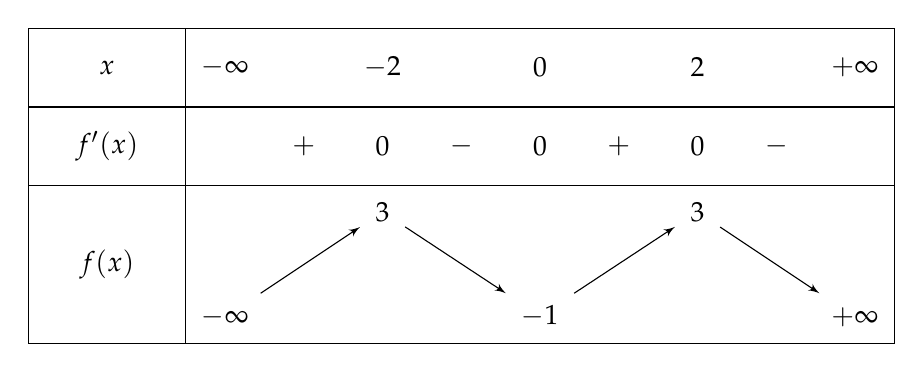
\begin{tikzpicture}
				\tkzTabInit[nocadre = false , lgt = 2 , espcl = 2]
					{ $ x $ / 1 , $ f'(x) $ / 1 , $ f(x) $ / 2 }
					{ $ - \infty $, $ -2 $ , $ 0 $ , $ 2 $ , $ + \infty $ } 
				\tkzTabLine
					{ , + , $ 0 $, - , $ 0 $, + , $ 0 $ , - , }
				\tkzTabVar
					{ -/ $ -\infty $ , +/ $ 3 $ , -/ $ -1 $ , +/ $ 3 $ , -/ $ +\infty $ }
			\end{tikzpicture}
	\end{center}
	\begin{multicols}{4}
		\begin{enumerate}
			\item[\textbf{A.}] $ 2 $
			\item[\textbf{B.}] $ 1 $
			\item[\textbf{C.}] $ 4 $
			\item[\textbf{D.}] $ 3 $
		\end{enumerate}
	\end{multicols}
	
\pagebreak

\textbf{Câu 12: } Trong không gian, cho hai véc tơ $ \overrightarrow{u} $ và $ \overrightarrow{v} $ thỏa mãn $\left| \overrightarrow{u} \right| = 5 $, $\left| \overrightarrow{v} \right| = 8 $ và $ \left( \overrightarrow{u}, \overrightarrow{v} \right) = 120\degree $. Khẳng định nào dưới đây là \textbf{đúng}?
	\begin{multicols}{2}
		\begin{enumerate}
			\item[\textbf{A.}] $ \overrightarrow{u}.\overrightarrow{v} = 20 $
			\item[\textbf{C.}] $ \overrightarrow{u}.\overrightarrow{v} = -20\sqrt{3} $
			\item[\textbf{B.}] $ \overrightarrow{u}.\overrightarrow{v} = -20 $
			\item[\textbf{D.}] $ \overrightarrow{u}.\overrightarrow{v} = 40 $
		\end{enumerate}
	\end{multicols}
\vspace{-0.75cm}
	
\textbf{Phần II. Câu trắc nghiệm đúng sai}

\textbf{Câu 1: } Cho hàm số $ y = \dfrac{x^2 + x + 7}{x - 1} $ 
\vspace{-0.5cm}
	\begin{enumerate}
		\item[\textbf{a)}] Đồ thị hàm số có hai điểm cực trị
		\item[\textbf{b)}] Hàm số đồng biến trên khoảng $ (-\infty; -2) $
		\item[\textbf{c)}] Đường tiệm cận xiên của đồ thị hàm số là đường thẳng $ y = x - 2 $ 
		\item[\textbf{d)}] Giá trị nhỏ nhất của hàm số trên khoảng $ (1; +\infty) $ bằng $ 9 $.
	\end{enumerate}	
	
\textbf{Câu 2: } Trong không gian $ Oxyz $, cho các điểm $ A(8;9;2) $, $ B(3;5;1) $ và $ C(11;10;4) $
\vspace{-0.5cm}
	\begin{enumerate}
		\item[\textbf{a)}] Điểm $ D $ thỏa mãn $ ABCD $ là hình bình hành có tọa độ là $ D(6;6;3) $
		\item[\textbf{b)}] Độ dài đường trung tuyến $ AM $ bằng $ \dfrac{\sqrt{14}}{2} $
		\item[\textbf{c)}] $ BAC = 30 \degree $
		\item[\textbf{d)}] Đường thẳng $ AB $ cắt mặt phẳng $ (Oxy) $ tại điểm $ N $ có tung độ là 1.
	\end{enumerate}

\textbf{Câu 3: } Cho hàm số $ y = f(x) = e^{x + \sqrt{16 - x^2}} $
\vspace{-0.5cm}
	\begin{enumerate}
		\item[\textbf{a)}] $ f'(x) = 0 $ có hai nghiệm phân biệt
		\item[\textbf{b)}] $ f(-4) = \dfrac{1}{e^4} $
		\item[\textbf{c)}] $ f'(x) = \left( 1 - \dfrac{x}{\sqrt{16 - x^2}} \right) e^{x + \sqrt{16 - x^2}} , \forall x \in [-4;4] $
		\item[\textbf{d)}] Tích của giá trị lớn nhất và giá trị nhỏ nhất của hàm số $ f(x) $ là $ e^{a + b\sqrt{c}} $ (với $ a,b,c \in \mathbb{Z} $ và $ c $ là số nguyên tố ). Khi đó $ a + 2b + 3c = 10 $
	\end{enumerate}

\textbf{Câu 4: } Một công ty bất động sản có 150 căn hộ cho thuê, biết rằng nếu cho thuê mỗi căn hộ với giá 2 triệu đồng mỗi tháng thì mỗi căn hộ đều có người thuê và cứ mỗi lần tăng giá cho thuê căn hộ thêm $ 100.000 $ dồng mỗi tháng thì có thêm 5 căn hộ bị bỏ trống. Xét các khẳng định sau:
\vspace{-0.5cm}
	\begin{enumerate}
		\item[\textbf{a)}] Khi giá cho thuê mỗi căn hộ là $ 2.200.000 $ đồng thì có 10 căn hộ bị bỏ trống
		\item[\textbf{b)}] Thu nhập cao nhất của công ty đạt được là $ 312.500.000 $ đồng
		\item[\textbf{c)}] Khi giá cho thuê mỗi căn hộ là $ 2.700.000 $ đồng thì thu nhập của công ty cao nhất
		\item[\textbf{d)}] Khi thu nhập công ty cao nhất thì căn hộ có người thuê là 5 căn hộ
	\end{enumerate}
	
\textbf{Phần III. Câu hỏi trắc nghiệm trả lời ngắn}

\textbf{Câu 1: } Cho biết máy bay $ A $ đang bay với vận tốc $ \overrightarrow{a} = (300;200;400) $ (đơn vị: km/h). Máy bay $ B $ bay cùng hướng và có tốc độ gấp ba lần tốc độ máy bay A. Tính tốc độ của máy bay $ B $ (làm tròn đến hàng đơn vị).

	\vspace{-0.5 cm}
	\textit{\textbf{Đáp số: }}
	\framebox[20mm]{\rule{0pt}{4mm}}
	
\textbf{Câu 2: } Một nhà máy sản xuất $ x $ sản phẩm trong mỗi tháng. Chi phí sản xuất $ x $ sản phẩm được cho bởi hàm chi phí $ C(x) = 16000 + 500x - 1,6x^2 + 0,004x^3 $ (nghìn đồng). Biết giá bán của mỗi sản phẩm là một hàm số phụ thuộc vào số lượng sản phẩm $ x $ và được cho bởi công thức $ p(x) = 1700 - 7x $ (nghìn đồng). Hỏi mỗi tháng nhà máy nên sản xuất bao nhiêu sản phẩm để lợi nhuận thu được là lớn nhất? Biết rằng kết quả khảo sát thị trường cho thấy sản phẩm sản xuất ra sẽ được tiêu thụ hết

	\textit{\textbf{Đáp số: }}
	\framebox[20mm]{\rule{0pt}{4mm}}
	
\textbf{Câu 3: } Đồ thị hàm số $ y = ax^3 + bx^2 + cx + d $ có hai điểm cực trị là $ A(1;-7), B(2;-8)$. Tính $y(-1)$

	\textit{\textbf{Đáp số: }}
	\framebox[20mm]{\rule{0pt}{4mm}}
	
\textbf{Câu 4: } Một người đứng ở mặt đất điều khiển hai flycam để phục vụ một chương trình của đài truyền hình. Flycam I ở vị trí $ A $ cách vị trí điều khiển $ 150 $ m về phía nam và $ 200 $ m về phía đông, đồng thời cách mặt đất $ 50 $ m. Flycam II ở vị trí $ B $ cách vị trí điều khiển $ 180 $ m về phía bắc và $ 240 $ m về phía tây, đồng thời cách mặt đất $ 60 $ m. Chọn hệ trục tọa độ $ Oxyz $ với gốc $ O $ là vị trí người điều khiển, mặt phẳng $ (Oxy) $ trùng với mặt đất, trục $ Ox $ có hướng trùng với hướng nam, trục $ Oy $ có hướng trùng với hướng đông, trục $ Oz $ vuông góc với mặt đất hướng lên bầu trờim đơn vị trên mỗi trục tính theo đơn vị mét. Khoảng cách giữa hai flycam đó bằng bao nhiêu mét (làm tròn kết quả đến hàng đơn vị)

	\textit{\textbf{Đáp số: }}
	\framebox[20mm]{\rule{0pt}{4mm}}

\textbf{Câu 5: } Một kỹ sư thiết kế mô hình trang trí cho một sân khấu nổi có dạng hình lập phương $ ABCD.A_1B_1C_1D_1 $ với độ dài các cạnh bằng $ 5 $ m. Để tạo ra nét độc đáo cho sân khấu, người kỹ sư muốn thiết kế một dàn đèn ánh sáng nối từ một điểm $ M $ trên đoạn thẳng $ AD_1 $ xuống một điểm $ N $ trên đoạn $ BD $ thỏa mãn $ AM = DN $. Dàn đèn ánh sáng có chiều dài ngắn nhất là bao nhiêu mét? (làm tròn kết quả đến hàng phần trăm) 

	\textit{\textbf{Đáp số: }}
	\framebox[20mm]{\rule{0pt}{4mm}}
	
\textbf{Câu 6: } Cho cầu thang gồm 10 bậc thang, biết mỗi lần đi chỉ có thể bước 1 hoặc 2 bậc. Hỏi có bao nhiêu cách để leo đến bậc thang thứ 10?

	\textit{\textbf{Đáp số: }}
	\framebox[20mm]{\rule{0pt}{4mm}}
	
\end{document}